\section{Measure-and-flip dynamic circuits are classical}\label{sec:classical}
\begin{lemma}[Classicality]\label{lem:classical}
Consider a circuit on qubits initialised to $|0\rangle$, with a layer of Hadamards on a subset $S$, followed by any sequence of (i)~permutation gates in the computational basis (X, CNOT, Toffoli, multi-controlled X), (ii)~diagonal gates, (iii)~computational-basis measurements and resets, and (iv)~classically controlled versions of (i)--(iii). The joint distribution of all measurement outcomes equals that of the classical algorithm that samples the bits in $S$ uniformly and applies (i), (iii), (iv) to bit strings.
\end{lemma}
\begin{proof}
Let $\Delta$ be complete dephasing in the computational basis. For a permutation $P$ and a diagonal unitary $D$, $\Delta(P\rho P^\dagger)=P\Delta(\rho)P^\dagger$ and $\Delta(D\rho D^\dagger)=\Delta(\rho)$; computational-basis measurement and reset commute with $\Delta$, and so do their classically controlled versions. Hence inserting $\Delta$ right after the Hadamard layer does not change any outcome statistics. Since $\Delta(|{+}\rangle\langle{+}|)=\mathbb{1}/2$, the state after dephasing is a uniform mixture over bit strings on $S$, evolved by permutations and measurements, i.e. a classical randomized algorithm.
\end{proof}
The lemma also applies at block level: a quantum adder acting on a register initialised to $|0\rangle$ is a permutation of basis states even if implemented with QFT rotations. \Cref{tab:classical} confirms the lemma on the two original proposals: a measure-and-flip 2-colouring of path graphs (simulated with the stabilizer method, $n$ up to 60) and a measure-and-flip subset-sum circuit with a QFT adder.

\begin{table}[t]\centering\small
\caption{Classicality check (Lemma~\ref{lem:classical}): success probability of the measure-and-flip circuits (stabilizer simulation, 50\,000 shots) versus the same rules executed classically ($2\times10^6$ trials); all differences are within $2\sigma$ of shot noise.}\label{tab:classical}
\begin{tabular}{lrrr}\toprule Circuit & iters & quantum & classical\\\midrule
2-col path P10 & 2 & 0.0086 & 0.0078\\
2-col path P10 & 5 & 0.0624 & 0.0624\\
2-col path P10 & 10 & 1.0000 & 1.0000\\
2-col path P10 & 20 & 1.0000 & 1.0000\\
2-col path P30 & 7 & 0.0000 & 0.0000\\
2-col path P30 & 15 & 0.0001 & 0.0001\\
2-col path P30 & 30 & 1.0000 & 1.0000\\
2-col path P30 & 60 & 1.0000 & 1.0000\\
2-col path P60 & 15 & 0.0000 & 0.0000\\
2-col path P60 & 30 & 0.0000 & 0.0000\\
\midrule \multicolumn{4}{l}{Subset sum $\{1,2,3,4\}$, target 7, QFT adder: TV distance 0.0008}\\
\bottomrule\end{tabular}
\end{table}

\section{Negation-forced preparation for CNF formulas}\label{sec:nf}
The main text builds the state $A_q$ from a general constraint automaton. This appendix is the original special case that motivated it: for a CNF formula, a clause is the negation of a forbidden pattern, and ``all other literals false'' is the condition that forces a variable. It gives the exact success probability, the PPZ-type gate bound and the ZX and fault-tolerant analyses below.
Let $F$ be a CNF formula over $x_1,\dots,x_n$ and $\pi$ an order of the variables.
\begin{definition}[Negative conditions]
For a variable $v$, let $\mathcal C_1(v)$ ($\mathcal C_0(v)$) be the clauses containing the literal $v$ ($\neg v$) whose other variables all precede $v$ in $\pi$. Given an assignment of the preceding variables, $v$ is \emph{forced to 1} (resp.\ 0) if some clause in $\mathcal C_1(v)$ ($\mathcal C_0(v)$) has all its other literals false. $\mathcal C^{K}$ keeps at most $K$ clauses of each polarity.
\end{definition}
\begin{definition}[In-place preparation $A_\pi^K$]
Process the variables in order $\pi$. For $v$: compute the flags $f_1,f_0$ (OR over clauses of the AND of their negated other literals), apply $\mathrm{CNOT}(f_1\!\to\!x_v)$, apply a Hadamard on $x_v$ controlled on $\neg f_1\wedge\neg f_0$, then uncompute the flags. All work qubits return to $|0\rangle$.
\end{definition}
The variable qubit is its own coin; no register of random choices and no history is stored. The circuit uses only Toffoli, controlled-Hadamard, CNOT and X gates (\cref{alg:prep}); the number of Toffolis is $O(\sum_v |\mathcal C(v)|\,k)=O(km)$.

\begin{algorithm}[t]
\caption{Negation-forced preparation $A^K_\pi$}\label{alg:prep}
\begin{algorithmic}[1]
\For{$v$ in order $\pi$}
\For{$c\in\mathcal C_1^K(v)\cup\mathcal C_0^K(v)$}
\State $a_c \gets \bigwedge_{\ell\in c\setminus\{v\}} \neg\ell$ \Comment{negative condition}
\EndFor
\State $f_1\gets\bigvee_{c\in\mathcal C_1}a_c$;\; $f_0\gets\bigvee_{c\in\mathcal C_0}a_c$
\State $x_v \mathrel{\oplus}= f_1$;\; \textbf{if} $\neg f_1\wedge\neg f_0$ \textbf{then} $H(x_v)$ \Comment{decision}
\State uncompute $f_1,f_0,a_c$
\EndFor
\end{algorithmic}
\end{algorithm}

\begin{figure}[t]\centering
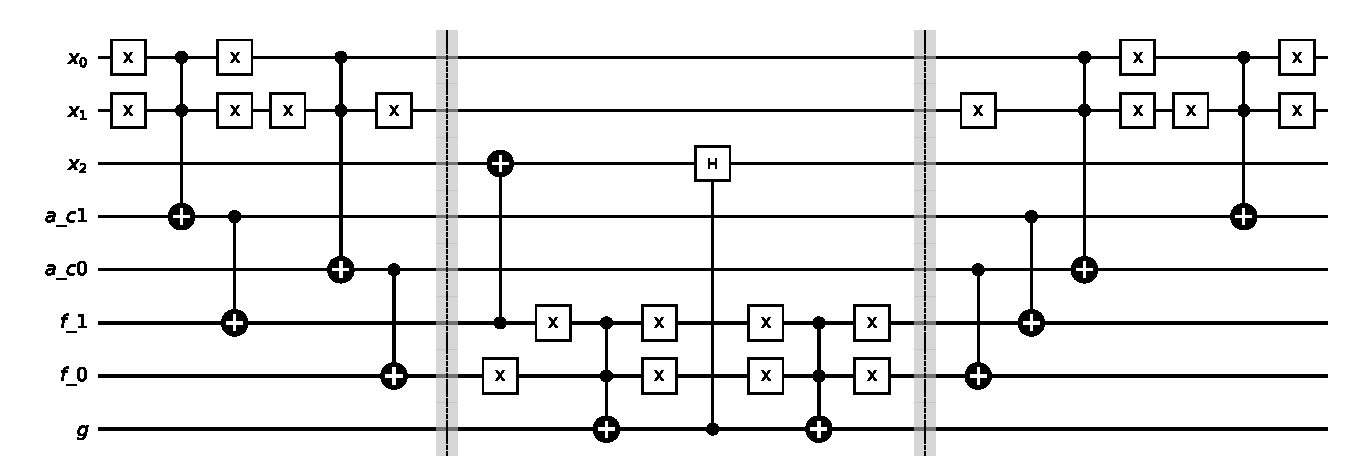
\includegraphics[width=\columnwidth]{figures/fig_step.pdf}
\caption{One negation-forced step for variable $x_2$ with clauses $(x_0\vee x_1\vee x_2)\in\mathcal C_1$ and $(\neg x_0\vee x_1\vee\neg x_2)\in\mathcal C_0$. Left: negative conditions $a_c$ (all other literals false) and flags $f_1,f_0$. Middle: forced value and the decision (controlled Hadamard on the variable itself). Right: uncomputation; all ancillas return to $|0\rangle$ and are reused for the next variable.}
\label{fig:step}
\end{figure}

\begin{lemma}[Soundness]\label{lem:sound}
If the variables preceding $v$ agree with a satisfying assignment $a$, then a forced value of $v$ equals $a_v$, and $v$ is never forced both ways.
\end{lemma}
\begin{proof}
If $c\in\mathcal C_1(v)$ has all other literals false under $a$, then $a$ satisfies $c$ only through the literal $v$, so $a_v=1$. Symmetrically for $\mathcal C_0(v)$. Both cannot hold.
\end{proof}

\begin{lemma}[Exact success probability]\label{lem:exact}
Let $D_\pi^K(a)$ be the number of unforced variables met when following $a$. Then
\begin{equation}
p_\pi^K=\big\|\Pi_{\mathrm{Sol}}A^K_\pi|0\rangle\big\|^2=\sum_{a\in\mathrm{Sol}}2^{-D^K_\pi(a)}.\label{eq:exact}
\end{equation}
Moreover $p^K_\pi$ is non-decreasing in $K$.
\end{lemma}
\begin{proof}
$A^K_\pi|0\rangle=\sum_x \alpha_x|x\rangle$ with $\alpha_x\ge 0$: each basis assignment $x$ is produced by a unique branch, whose amplitude is $2^{-1/2}$ per Hadamard applied to $|0\rangle$ and $1$ per forced step (all ancillas are restored). By \cref{lem:sound} every solution $a$ is reachable, its branch follows $a$, and $\alpha_a^2=2^{-D^K_\pi(a)}$. Increasing $K$ enlarges the sets of forcing clauses, so $D^K_\pi(a)$ can only decrease.
\end{proof}
\Cref{eq:exact} reduces the computation of $p_\pi$ to model enumeration and is what makes our large-$n$ numerics exact. We verified it against exhaustive branch enumeration (zero discrepancy on all tested instances) and against circuit simulation (\cref{sec:exp}).

\begin{theorem}[Gate complexity]\label{thm:main}
Let $F$ be a $k$-CNF with $n$ variables and $m$ clauses and a unique solution. Amplitude amplification over $A_\pi$ with random orders and an unknown-probability schedule~\cite{bbht1998,bhmt2002} finds the solution with $O\!\big(n\,2^{((1-1/k)n+1)/2}\big)$ expected applications of $A_\pi$, $A_\pi^\dagger$ and the phase oracle, i.e.\ $O^*(2^{(1-1/k)n/2})$ gates, using $n+O(m)$ qubits.
\end{theorem}
\begin{proof}
By \cref{lem:exact}, $p_\pi\ge 2^{-D_\pi(a^*)}$. The satisfiability coding lemma of PPZ~\cite{ppz1999} gives $\mu=\mathbb E_\pi[D_\pi(a^*)]\le(1-1/k)n$. By Markov's inequality $\Pr_\pi[D_\pi(a^*)<\mu+1]\ge 1/(\mu+1)$, so after an expected $O(n)$ random orders one has $p_\pi\ge2^{-(\mu+1)}$; for each order, amplitude amplification with an exponential schedule capped at $O(2^{(\mu+1)/2})$ rounds succeeds with constant probability~\cite{bbht1998}. Each application of $A_\pi$ or the oracle costs $O(km)$ Toffolis.
\end{proof}
For several solutions, \cref{eq:exact} sums over all of them and the bound only improves. The PPZ exponent is not new~\cite{ambainis2004,dunjko2018}; what \cref{lem:exact} adds is an exact, cheaply computable probability for \emph{every} instance and every condition budget $K$, which enables the selection procedure of \cref{sec:zx}.

\section{ZX-calculus co-design}\label{sec:zx}
\paragraph{Pipeline.} Each component---$A_\pi^K$, the phase oracle $O_F$ (clause ANDs, a global AND, a $Z$), and the reflection $S_0$---is compiled to Clifford+$T$, converted to a ZX-diagram, simplified with \texttt{full\_reduce} and re-extracted~\cite{duncan2020,pyzx}. Compute/uncompute pairs of Toffolis that share controls fuse into phase gadgets, which is where most $T$ gates disappear.
\paragraph{Verification.} Every optimised component is checked against the original: exactly with statevectors for small instances, and for larger ones by running $U_{\rm orig}U_{\rm ZX}^\dagger$ on random inputs (with a Hadamard to expose relative phases) under MPS simulation and requiring that every shot returns the input.
\paragraph{Condition selection.} Checking more negative conditions raises $p^K_\pi$ (\cref{lem:exact}) but makes $A^K_\pi$ more expensive. With $G(\cdot)$ the post-ZX $T$-count,
\begin{equation}
\begin{aligned}\mathcal T(K)&=\frac{\pi}{4\sqrt{p^K_\pi}}\big(2G(A^K_\pi)+G(O_F)+G(S_0)\big),\\ K^*&=\arg\min_K\mathcal T(K).\end{aligned}\label{eq:select}
\end{equation}
Both factors are computable without running the quantum algorithm: $p^K_\pi$ via \cref{eq:exact} and $G$ via ZX simplification.

\section{Experiments on CNF and colouring instances}\label{sec:exp}
\paragraph{Setup.} Families: random 3-SAT at clause density $4.2$, random 4-SAT at $9.6$, positive 1-in-3-SAT with $0.6n$ triples (encoded as one 3-clause and three 2-clauses each), and Erd\H{o}s--R\'enyi graph 3-colouring with two bits per vertex (average degree $4.2$, or $3.0$ below 10 vertices). Only satisfiable instances are kept; solutions are enumerated with MiniSat~\cite{minisat} through PySAT~\cite{pysat} (instances with more than $2\times10^4$ solutions are rejected). Circuits are built in Qiskit~\cite{qiskit2024}; MPS simulations~\cite{vidal2003} use Qiskit Aer; ZX optimisation uses PyZX~\cite{pyzx}. All runs used two CPU cores.

\paragraph{E1: circuit-level validation with MPS.} \Cref{fig:mps} compares the success probability of the simulated circuit $A_\pi|0\rangle$ with \cref{eq:exact} for \NMPSA{} instances with $n$ up to \MaxMPSn{} (up to \MaxMPSQubits{} qubits), and the success probability after $k^*$ full amplification rounds with the prediction $\sin^2((2k^*+1)\arcsin\sqrt p)$, for both the negation-forced preparation and Grover's uniform preparation. \MPSAgreement{} Runs exceeding 15 minutes were stopped (preparation: 3-COL at $n=20,24$ and 3-SAT at $n=24$; amplification: the uniform baseline for 4-SAT and beyond $n=8$): the MPS bond dimension grows with $n$ and the number of rounds, which limits the validation, not the algorithm.

\begin{figure}[t]\centering
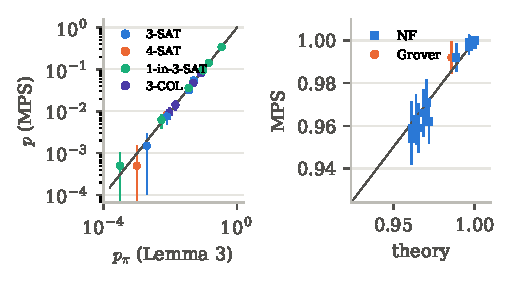
\includegraphics[width=\columnwidth]{figures/fig_mps.pdf}
\caption{\orig{ideal matrix-product-state simulation} MPS circuit simulations versus theory. Left: success probability of $A_\pi|0\rangle$ (one point per instance; error bars are $2\sigma$ shot noise). Right: success after $k^*$ amplification rounds for negation-forced (NF) and uniform (Grover) preparations; the label gives $k^*$.}
\label{fig:mps}
\end{figure}

\paragraph{E2: scaling across problem families.} \Cref{fig:scaling} and \cref{tab:scaling} report $\log_2 p$ versus $n$ for \NInstances{} instances (10 per size, 10 random orders each). Fitting $p\propto2^{-sn}$ with bootstrap confidence intervals, the effective quantum base $2^{s/2}$ drops from \GroverBaseRange{} for the uniform preparation to \NFBaseRange{} with negative conditions. The measured fraction of decisions per variable stays below the PPZ bound $1-1/k$ (\cref{tab:scaling}).

\begin{figure*}[t]\centering
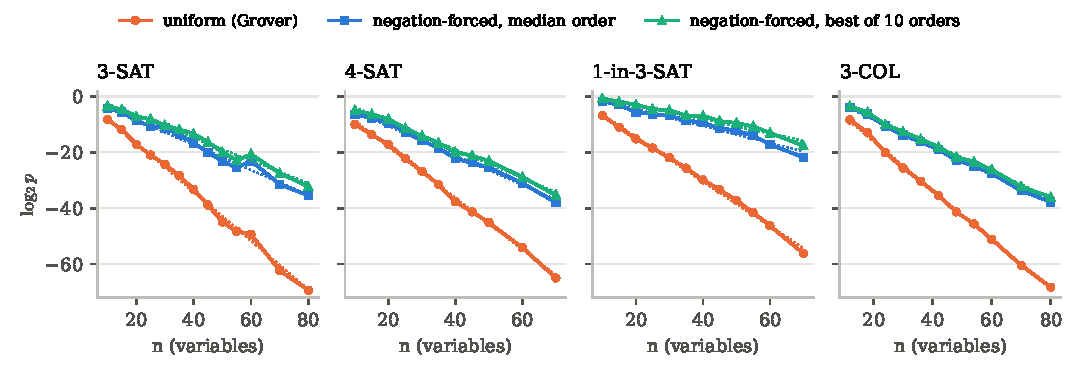
\includegraphics[width=0.95\textwidth]{figures/fig_scaling.pdf}
\caption{\orig{ideal matrix-product-state simulation} Success probability of the prepared state versus number of variables (median over 10 instances per size; dotted lines: least-squares fits). Orange: uniform superposition (Grover). Blue/green: negation-forced preparation, median and best of 10 variable orders.}
\label{fig:scaling}
\end{figure*}
\begin{table}[t]\centering\small
\caption{Fitted scaling $p\propto 2^{-sn}$ (95\% bootstrap CI) and effective quantum base $2^{s/2}$; decisions per variable $D/n$ along solutions versus the PPZ bound $1-1/k$ (for $k$-CNF).}\label{tab:scaling}
\resizebox{\columnwidth}{!}{\begin{tabular}{lrcccc}\toprule Family & inst. & Grover & NF (median) & NF (best) & $D/n$ (bound)\\\midrule
3-SAT & 130 & 1.355 & 1.169 [1.161,1.177] & 1.152 & 0.589 (0.667)\\
4-SAT & 110 & 1.375 & 1.200 [1.191,1.208] & 1.192 & 0.628 (0.750)\\
1-in-3-SAT & 120 & 1.318 & 1.110 [1.103,1.117] & 1.093 & 0.511 (--)\\
3-COL & 110 & 1.357 & 1.187 [1.182,1.192] & 1.181 & 0.630 (--)\\
\bottomrule\end{tabular}}
\end{table}

\paragraph{E3: ZX simplification.} \Cref{tab:zx} lists $T$ and two-qubit gate counts per component before and after ZX simplification, together with the equivalence checks. \ZXSummary{} For 4-SAT, PyZX extraction of the oracle (77 four-literal clauses) did not finish within one CPU-hour; ZX extraction cost is a practical limitation of the approach at this size.

\begin{table}[t]\centering\small
\caption{ZX simplification per component (mean over instances): $T$-count and two-qubit gates before $\to$ after, and the equivalence checks (statevector or MPS, see text).}\label{tab:zx}
\begin{tabular}{llrrr}\toprule Family & comp. & $T$ & 2q & $\Delta T$\\\midrule
3-SAT & $A_\pi$ & 1338$\to$536 & 1153$\to$1325 & $-60\%$\\
3-SAT & $O_F$ & 2618$\to$1130 & 2244$\to$2991 & $-57\%$\\
3-SAT & $S_0$ & 182$\to$56 & 157$\to$117 & $-69\%$\\
1-in-3-SAT & $A_\pi$ & 473$\to$205 & 448$\to$555 & $-57\%$\\
1-in-3-SAT & $O_F$ & 1036$\to$417 & 888$\to$925 & $-60\%$\\
1-in-3-SAT & $S_0$ & 182$\to$56 & 157$\to$117 & $-69\%$\\
3-COL & $A_\pi$ & 1737$\to$859 & 1506$\to$2064 & $-51\%$\\
3-COL & $O_F$ & 2688$\to$865 & 2304$\to$2166 & $-68\%$\\
3-COL & $S_0$ & 238$\to$72 & 205$\to$130 & $-70\%$\\
\bottomrule\end{tabular}
\\[2pt]\footnotesize Equivalence checks passed: 9/9 components.
\end{table}

\paragraph{E4: selecting negative conditions.} \Cref{fig:select} shows $\mathcal T(K)$ from \cref{eq:select} for $K\in\{0,1,2,3,\infty\}$, where $K=0$ is Grover's algorithm. \SelectSummary{}

\begin{figure}[t]\centering
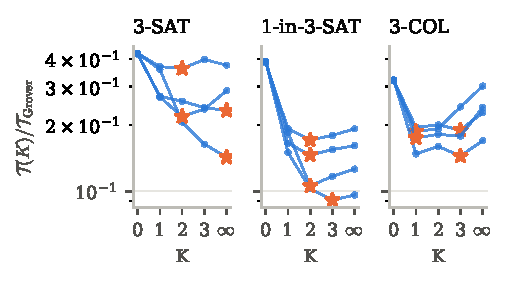
\includegraphics[width=\columnwidth]{figures/fig_select.pdf}
\caption{\orig{resource estimate (model)} Total expected $T$-count (\cref{eq:select}, after ZX) versus the number of negative conditions $K$ checked per variable and polarity, normalised by Grover ($K=0$, no ZX). Each line is one instance; stars mark $K^*$.}
\label{fig:select}
\end{figure}

\paragraph{E5: fault-tolerant resources and classical baselines.} We count logical $T$ gates of the generated circuits exactly for $n$ up to 80, combine them with the median $p$ from E2, and estimate surface-code resources~\cite{fowler2012,litinski2019} with physical error rate $10^{-3}$, threshold $10^{-2}$, logical error $p_L(d)=0.1(p/p_{\rm th})^{(d+1)/2}$, a total failure budget of $1\%$, one 15-to-1 factory~\cite{bravyi2005} and a $1\,\mu$s code cycle; ZX ratios from E3 are applied as measured averages per component (for 4-SAT, the average over the other families). \Cref{tab:resources} reports the result. \ResourceSummary{}

\begin{table*}[t]\centering\small
\caption{Fault-tolerant estimates for the median instance: expected logical $T$-count to find a solution, surface-code distance $d$, physical qubits and runtime (model in the text). Classical reps.: expected repetitions $1/p$ of the classical algorithm with the same negative conditions.}\label{tab:resources}
\begin{tabular}{lr|rrrr|rrrr|r}\toprule
 & & \multicolumn{4}{c|}{Grover (uniform)} & \multicolumn{4}{c|}{Negation-forced + ZX} & \\
Family & $n$ & $T$ & $d$ & qubits & time & $T$ & $d$ & qubits & time & classical reps.\\\midrule
3-SAT & 40 & 1.0e9 & 29 & 9.7e5 & 8.2\,h & 2.5e6 & 23 & 6.1e5 & 58.1\,s & 1.0e5\\
3-SAT & 80 & 5.3e14 & 41 & 3.8e6 & 690.3\,y & 3.1e9 & 29 & 1.9e6 & 1.0\,d & 3.9e10\\
4-SAT & 40 & 1.4e10 & 31 & 2.3e6 & 5.1\,d & 6.4e7 & 27 & 1.8e6 & 28.8\,min & 4.8e6\\
4-SAT & 70 & 3.2e14 & 41 & 7.2e6 & 420.4\,y & 2.6e10 & 33 & 4.6e6 & 10.0\,d & 2.6e11\\
1-in-3-SAT & 40 & 1.4e8 & 25 & 4.4e5 & 58.7\,min & 8.3e4 & 19 & 2.5e5 & 1.6\,s & 6.5e2\\
1-in-3-SAT & 70 & 2.3e12 & 35 & 1.5e6 & 2.6\,y & 1.0e7 & 23 & 6.4e5 & 3.8\,min & 3.3e6\\
3-COL & 30 & 6.0e7 & 25 & 4.8e5 & 25.2\,min & 9.4e5 & 21 & 3.4e5 & 19.7\,s & 1.5e4\\
3-COL & 80 & 4.2e14 & 41 & 3.4e6 & 552.7\,y & 1.0e10 & 31 & 1.9e6 & 3.6\,d & 2.4e11\\
\bottomrule\end{tabular}
\end{table*}
\paragraph{Scope and limits of these results.} The gains are relative to Grover's uniform preparation and are quadratic relative to the classical randomized algorithm that uses the same negative conditions (\Cref{tab:resources}, column ``classical reps.''). They are \emph{not} gains over industrial CDCL solvers: MiniSat solved every instance in our study with at most \MiniSatMaxConflicts{} conflicts. Random instances near the threshold are easy for CDCL at these sizes; our numerics measure exponents, not practical runtimes. Negative conditions do not reduce the number of logical qubits by themselves, since the oracle's clause register dominates; the physical-qubit savings come from fewer gates, which permits a smaller code distance. The algorithm is Las Vegas, so an error costs a repetition but never yields a wrong answer; this is error \emph{detection} at the algorithmic level, not fault tolerance. ZX optimisation and full amplification were simulated only for small instances, the large-$n$ resource estimates combine exact gate counts with ZX ratios measured at small $n$, and the surface-code model is deliberately simple. Stronger negative conditions (PPSZ-style implications via bounded-width resolution) fit the same framework, and \cref{lem:exact} still applies whenever forced values are sound.

\section{Unknown success probability: heralded weak measurement}\label{app:herald}
Theorem~\ref{thm:main} uses an exponential schedule because $p_\pi$ is unknown. On dynamic-circuit hardware an alternative is to copy the satisfaction flag weakly to a herald qubit inside every oracle call ($\mathrm{CR}_y(2\varphi_t)$, no extra queries) and measure it before the reflection; a click projects onto the solution subspace and certifies the answer before readout~\cite{mizel2009,andres2022,prabhat2026}. With the schedule $\sin^2\varphi_t=\min(1/2,5/(t+1))$ the expected cost approaches $1.01\sqrt{N/M}$ without knowing $M$, versus $\approx1.45\sqrt{N/M}$ for BBHT (\cref{tab:herald}); the 2-D model was validated against full circuit simulations. The same schedule applies verbatim to amplification over $A_\pi$ with $N/M$ replaced by $1/p_\pi$.
\begin{table}[h]\centering\small
\caption{Expected oracle queries to a verified solution, in units of $\sqrt{N/M}$ (2-D model, exact). Heralded: weak measurement of the satisfaction flag with $\sin^2\varphi_t=\min(1/2,5/(t+1))$, no knowledge of $M$.}\label{tab:herald}
\begin{tabular}{rccc}\toprule $\log_2(N/M)$ & Grover ($M$ known) & BBHT & Heralded\\\midrule
6 & 0.88 & 1.60 & 0.78\\
10 & 0.81 & 1.63 & 1.00\\
14 & 0.79 & 1.52 & 1.02\\
18 & 0.79 & 1.48 & 1.01\\
22 & 0.79 & 1.44 & 1.01\\
24 & 0.79 & 1.43 & 1.01\\
\bottomrule\end{tabular}
\end{table}

\section{Noisy intermediate-scale simulation}\label{app:noise}
For completeness, \cref{tab:noise} reports a small instance under the \texttt{FakeFez} noise model with relaxation charged to every mid-circuit measurement. At $N=16$ all methods are at the noise floor (cost $\approx8$, equal to guessing and verifying); measurement-based uncomputation (MBU: ancillas uncomputed by $X$-basis measurement and classically controlled phase fixes~\cite{gidney2018}), which needs many mid-circuit measurements, degrades sharply with latency. ``Textbook'' uses Qiskit's multi-controlled gates; ``coherent-rccx'' uses relative-phase Toffolis; ``Heralded $T$'' is the scheme of \cref{app:herald} with at most $T$ iterations. The advantages of the CNF special case discussed here therefore concern query and gate complexity in the fault-tolerant regime, not present-day hardware.
\begin{table}[h]\centering\small
\caption{Noisy simulation with the \texttt{FakeFez} (IBM Heron) noise model, binary $2\times2$ Sudoku ($N=16$, $M=2$); $L$: idle relaxation added per mid-circuit measurement. Cost: oracle queries per valid solution (random guessing: 8). Cert.: $P(\text{valid}\mid\text{herald click})$.}\label{tab:noise}
\begin{tabular}{lrrrr}\toprule Method & $L$ (ns) & $P$(valid) & cert. & cost\\\midrule
Grover textbook & 0 & 0.401 & -- & 7.5\\
Grover coherent-rccx & 0 & 0.358 & -- & 8.4\\
Grover MBU-rccx & 0 & 0.421 & -- & 7.1\\
Heralded T=2 & 0 & 0.380 & 0.67 & 7.0\\
Heralded T=4 & 0 & 0.339 & 0.57 & 11.3\\
Heralded T=6 & 0 & 0.336 & 0.49 & 14.0\\
Grover textbook & 2000 & 0.401 & -- & 7.5\\
Grover coherent-rccx & 2000 & 0.358 & -- & 8.4\\
Grover MBU-rccx & 2000 & 0.102 & -- & 29.3\\
Heralded T=2 & 2000 & 0.340 & 0.60 & 7.9\\
Heralded T=4 & 2000 & 0.308 & 0.51 & 12.5\\
Heralded T=6 & 2000 & 0.297 & 0.43 & 16.1\\
\bottomrule\end{tabular}
\end{table}
